\section{Real-Setup Experiments}

\subsection{Real-Setup Test Plan}

After validating the controllers in simulation, preliminary real-setup
experiments were carried out to investigate their transfer to the physical
unbalanced-disk system. The purpose of these tests was not to obtain a fully
optimized hardware demonstration, but to identify practical effects that are
not present in simulation, such as sensor bias, voltage limitations,
state-estimation errors, and safety constraints.

The real setup was accessed through
\texttt{gym\_unbalanced\_disk.UnbalancedDisk\_exp}. The sampling time was
\begin{equation}
    T_s = 0.025~\mathrm{s}.
\label{eq:real_sampling_time}
\end{equation}
The hardware interface allows the assignment voltage range
\begin{equation}
    u_k \in [-3,3]~\mathrm{V}.
\label{eq:real_voltage_range}
\end{equation}
However, conservative voltage limits were used during the first hardware tests
for safety. In the DQN safe deployment test, the applied input was clipped to
\begin{equation}
    u_k \in [-2,2]~\mathrm{V},
\label{eq:real_dqn_safe_voltage}
\end{equation}
which made the real experiment more restrictive than the simulation training
environment.

A practical issue was the angular velocity measurement. The raw velocity signal
showed noticeable bias and noise, so it was recorded for analysis but not used
directly for feedback. Instead, the controller used a filtered finite-difference
estimate from the measured angle,
\begin{equation}
\begin{aligned}
    \omega_{\mathrm{est},k}
    =
    \alpha \omega_{\mathrm{est},k-1}
    +
    (1-\alpha)
    \frac{\mathrm{wrap}(\theta_k-\theta_{k-1})}{T_s}.
\end{aligned}
\label{eq:real_velocity_estimate}
\end{equation}
The filter coefficient was set to \(\alpha=0.80\).
Safety checks were included to stop the experiment if the unwrapped angle or
estimated angular velocity exceeded predefined limits. The logged signals
included the measured angle, estimated velocity, raw velocity, applied voltage,
wrapped upright error, and controller action or mode information.

Therefore, the real-setup experiments should be interpreted as safe preliminary
deployment tests. Their main role is to evaluate simulation-to-real transfer
and identify the practical limitations that prevent direct deployment of the
simulation-trained controllers.



\subsection{Real-Setup DQN Safe Deployment}

The first controller tested on the real setup was the DQN swing-up policy
trained in simulation. The same sine-cosine state representation was used, but
the angular velocity was replaced by the filtered estimate
\(\omega_{\mathrm{est}}\) obtained from the measured angle. The original DQN
action set contained voltages up to \(\pm 3\) V, but during the first safe
hardware deployment the selected action was clipped to \([-2,2]\) V. This
reduced the risk to the setup, but also made the real experiment more
restrictive than the simulation training environment.

Figure~\ref{fig:real_dqn_theta_input} shows the measured angle and applied
input during the real DQN safe test. The disk moved only to a small offset from
the downward equilibrium and did not approach the upright position
\(\theta=\pm\pi\). At the same time, the applied input remained close to the
positive safety limit of \(+2\) V for most of the rollout. This indicates that
the policy repeatedly selected a large positive action that was clipped by the
real-system safety bound. As a result, the controller behaved almost like a
constant-voltage input rather than a feedback policy that successfully adapted
during swing-up.

\begin{figure}[H]
    \centering
    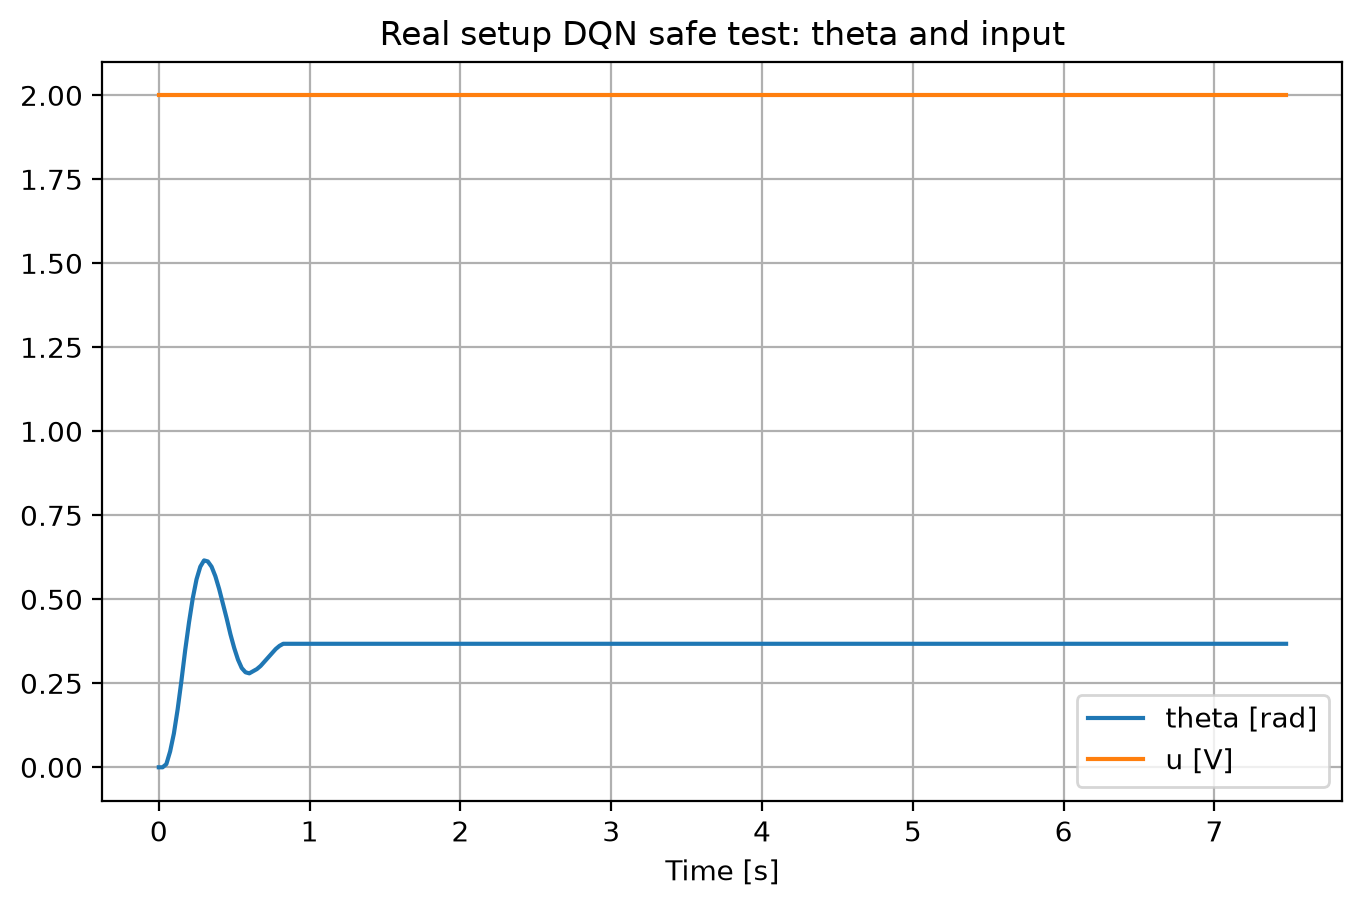
\includegraphics[width=0.75\linewidth]{figures/real_dqn_safe_theta_input.png}
    \caption{Measured angle and applied input during the real-setup DQN safe
    deployment test. Input remains close to the \(+2\) V safety limit, while
    the disk fails to reach the upright position.}
    \label{fig:real_dqn_theta_input}
\end{figure}

The result should therefore be interpreted as an unsuccessful direct transfer
from simulation to hardware. The conservative voltage clipping is one important
reason: the DQN was trained with actions up to \(\pm 3\) V, while the real test
allowed only \(\pm 2\) V, reducing the available swing-up energy. In addition,
the real setup differs from the simulator because of friction, delay, actuator
behavior, sensor noise, and velocity-estimation errors. The raw angular
velocity measurement showed bias and noise, so the controller used an
angle-based filtered estimate instead. This changed the state distribution seen
by the DQN policy and likely contributed to the nearly constant-action behavior
observed in the real experiment.


\subsection{Real-Setup Hybrid RBF Policy Test}

The second controller tested on the real setup was the optimized hybrid
energy-pumping and RBF policy. The real implementation used three modes:
Energy, Brake, and RBF. The Energy mode was used for swing-up energy injection,
the Brake mode was added to reduce excessive angular velocity near the upright
region, and the RBF mode was used for local stabilization. For safety, the
voltage limits were set to \(\pm 2.0\) V in Energy mode, \(\pm 0.5\) V in Brake
mode, and \(\pm 1.2\) V in RBF mode. As in the DQN real-setup test, the raw
angular velocity was recorded only for analysis, while the feedback velocity
was estimated from the measured angle because of bias and noise in the raw
sensor signal.

Figure~\ref{fig:real_hybrid_theta} shows the measured angle during the real
hybrid RBF test. Compared with the real DQN safe deployment, the hybrid
controller generated much larger disk motion and approached the upright region
several times. This shows that the energy-pumping part transferred better to
the physical setup. However, the disk still continued to oscillate with large
amplitude and did not achieve sustained upright stabilization. Thus, the real
hybrid policy achieved partial transfer: it could generate swing-up motion, but
the capture and local stabilization phase was not robust enough on the real
setup.

\begin{figure}[H]
    \centering
    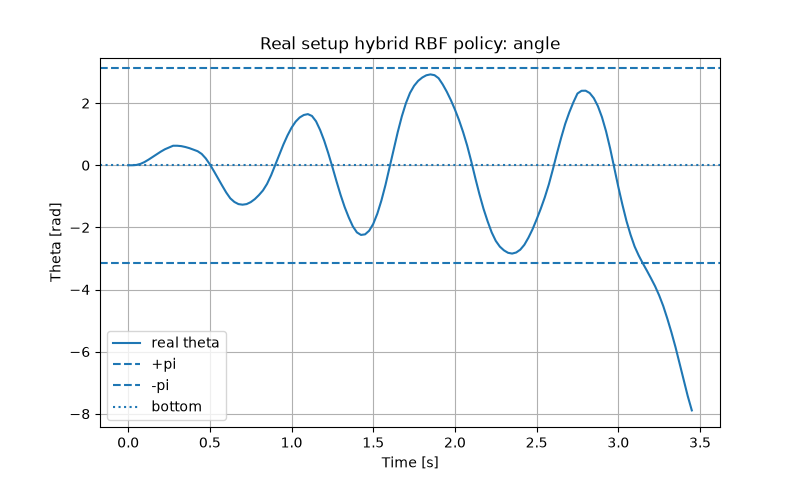
\includegraphics[width=0.75\linewidth]{figures/real_hybrid_rbf_theta.png}
    \caption{Angle response of the real-setup hybrid RBF policy. The controller
    approaches the upright region but does not achieve sustained stabilization.}
    \label{fig:real_hybrid_theta}
\end{figure}

The input and mode behavior in Fig.~\ref{fig:real_hybrid_input_mode} explain
the failed capture. The input frequently reaches the Energy-mode limits,
showing that the controller relies mainly on energy pumping. Meanwhile, the
mode signal shows that Brake and RBF modes are only activated briefly near the
upright region. Therefore, the main issue is not the lack of swing-up energy,
but the inability to remain in the local stabilization modes long enough to
capture the disk near the upright equilibrium.

\begin{figure}[H]
    \centering
    \begin{subfigure}[t]{0.48\linewidth}
        \centering
        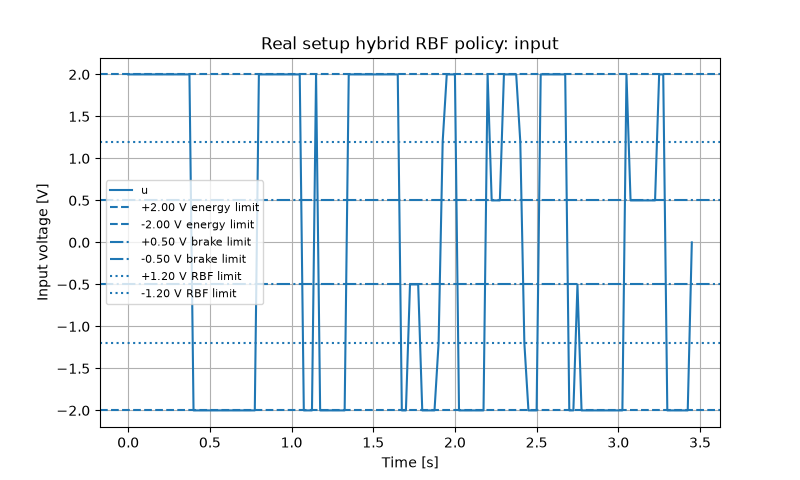
\includegraphics[width=\linewidth]{figures/real_hybrid_rbf_input.png}
        \caption{Applied input voltage.}
        \label{fig:real_hybrid_input}
    \end{subfigure}
    \hfill
    \begin{subfigure}[t]{0.49\linewidth}
        \centering
        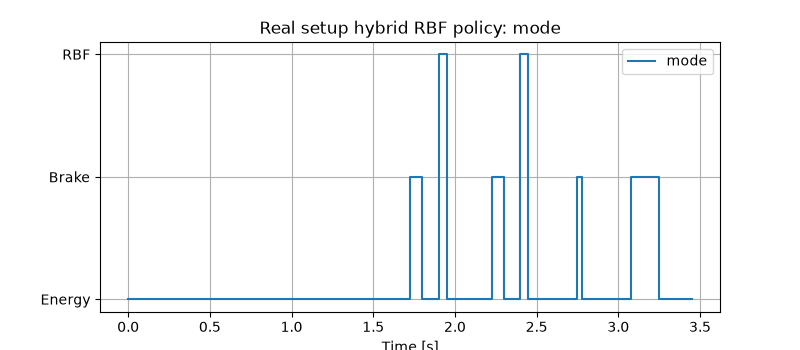
\includegraphics[width=\linewidth]{figures/real_hybrid_rbf_mode.png}
        \caption{Control mode.}
        \label{fig:real_hybrid_mode}
    \end{subfigure}
    \caption{Input and mode behavior of the real-setup hybrid RBF policy.}
    \label{fig:real_hybrid_input_mode}
\end{figure}

This behavior is likely caused by the limited authority of the Brake and RBF
modes and the sensitivity of the switching logic to velocity estimation, noise,
and real-system mismatch. Since the switch to Brake or RBF mode depends on the
wrapped upright error and estimated angular velocity, an inaccurate or delayed
velocity estimate can cause the controller to enter the local stabilization
region too early, too late, or for too short a time. Overall, the real hybrid
RBF controller transferred better than the real DQN policy in terms of energy
generation, but reliable upright capture still requires further real-system
tuning of the switching conditions and local stabilizer.


\subsection{Discussion of Simulation-to-Real Gap}

The real setup experiments revealed a clear simulation-to-real gap. In
simulation, both the DQN controller and the optimized hybrid RBF controller
achieved successful swing-up and stabilization. On the physical setup, however,
the DQN controller did not generate sufficient swing-up motion, while the
hybrid RBF controller produced large oscillations but failed to reliably capture
and stabilize the disk near the upright position.

For the DQN controller, the main issue was the mismatch between the simulation
training conditions and the safe hardware deployment. The policy was trained
with actions up to \(\pm 3\) V, but the real experiment clipped the applied
voltage to \(\pm 2\) V. This reduced the available swing-up energy and caused
the input to remain close to the positive safety limit without producing enough
motion to reach the upright region. In addition, the real setup used a filtered
angle-based velocity estimate instead of the clean simulated velocity, which
changed the state distribution seen by the neural network.

The hybrid RBF controller showed better partial transfer because its
energy-pumping component could excite the disk and bring it close to the
upright region. However, the capture phase was not robust enough. The Brake and
RBF modes had smaller safety-limited voltages, and the switching logic depended
on the estimated angular velocity. Therefore, velocity-estimation errors,
sensor noise, delay, friction, and actuator mismatch could cause the controller
to enter the local stabilization modes at unsuitable times or for too short a
duration.

Overall, the real experiments show that successful simulated swing-up does not
guarantee direct hardware transfer. The DQN test highlights the sensitivity of
learned value-based policies to voltage limits and state-distribution changes,
while the hybrid RBF test shows that physical insight improves energy
generation but does not by itself guarantee robust capture. Future work should
focus on safer but less restrictive voltage scheduling, better angular-velocity
calibration, real-setup retuning of switching thresholds and local gains, and
training with domain randomization or real-system data.
